\documentclass{article}

\usepackage{siunitx}
\usepackage{amsmath}
\usepackage{amssymb}
\usepackage[letterpaper]{geometry}
\usepackage{graphicx}

\title{4125 HW 6}
\author{Duncan Wilkie}
\date{3 April 2022}

\begin{document}

\maketitle

\section*{5.16}
By the chain rule, considering $V$ to be a function of $P$ and $T$ through some equation of state,
\[dV=\left( \frac{\partial V}{\partial T}\right)_{N,P}dT+\left( \frac{\partial V}{\partial P} \right)_{N,T}dP=\left( \frac{\partial V}{\partial T} \right)_{N,P}dT-V\kappa_{T}dP\]
Similarly, we may consider $T$ a function of $P$ and $S$ through an equation of state and an entropy-state relation to eliminate volume, yielding through the chain rule
\[dV=\left( \frac{\partial V}{\partial T} \right)_{N,P}\left(\left[ \frac{\partial T}{\partial P} \right]_{N,S}dP+\left[ \frac{\partial T}{\partial S}\right]_{N,T}dS  \right)-V\kappa_{T}dP\]
Presuming $dS=0$, since something isentropic needs to show up to get the isentropic compressibility out,
\[dV=\left( \frac{\partial V}{\partial T} \right)_{N,P}\left( \frac{\partial T}{\partial P} \right)_{N,S}dP-V\kappa_{T} dP\]
\[\Leftrightarrow \left( \frac{\partial V}{\partial P} \right)_{N,S}=\left( \frac{\partial V}{\partial T} \right)_{N,P}\left( \frac{\partial T}{\partial P} \right)_{N,S}-V\kappa_{T}\]
There is a Maxwell relation
\[\left( \frac{\partial T}{\partial P} \right)_{N,S}=\left( \frac{\partial V}{\partial S} \right)_{N,P}\]
which one can relate to the thermal expansion as
\[\left( \frac{\partial V}{\partial S} \right)_{N,P}=\left( \frac{\partial V}{\partial T} \right)_{N,P}\left( \frac{\partial T}{\partial S} \right)_{N,P}=V\beta\left( \frac{\partial T}{\partial S} \right)_{N,P}\]
\[\Rightarrow \left( \frac{\partial V}{\partial P} \right)_{N,S}=\left( \frac{\partial V}{\partial T} \right)_{N,P}V\beta\left( {\frac{\partial T}{\partial S}} \right)_{N,P}-V\kappa_{T}\]
The heat capacity at constant pressure may be written $C_{P}=T\left( \frac{\partial S}{\partial T} \right)_{N,P}$, so we obtain
\[-V\kappa_{S}=(\beta V)\left(\beta V\frac{T}{C_{P}}\right)-V\kappa_{T}\]
\[\Leftrightarrow \kappa_{T}=\kappa_{S}+\frac{TV\beta^{2}}{C_{P}}\]

\section*{5.20}
The Helmholtz free energy is defined as
\[F=U-TS\]
For an internal energy of $\SI{10.2}{eV}=\SI{1.63e-18}{J}$ and an entropy of $(\SI{1.38e-23})\ln 4=\SI{1.91e-23}{J/K}$, this expression changes sign at
\[T=\frac{U}{S}=\frac{\SI{1.63e-18}{J}}{\SI{1.91e-23}{J/K}}=\SI{85000}{K}\]
Temperatures above this value have negative $F$; those below positive.

\section*{5.23a}
By the chain rule,
\[d\Phi=dU-d(TS)-d(\mu N)=dU-SdT-TdS-\mu dN-Nd\mu\]
By the fundamental thermodynamic identity,
\[d\Phi= TdS-PdV+\mu dN-SdT-TdS-\mu dN-Nd\mu\]
\[=-PdV-SdT-Nd\mu\]
At constant volume and temperature,
\[N=-\left( \frac{\partial \Phi}{\partial \mu} \right)_{V,T}\]
At constant volume and chemical potential,
\[S=-\left( \frac{\partial \Phi}{\partial T} \right)_{V,\mu}\]
At constant temperature and chemical potential,
\[P=-\left( \frac{\partial \Phi}{\partial V} \right)_{T,\mu}\]

\section*{5.23b}
Since the system is in thermal and diffusive equillibrium, $dT=d\mu=0$. Pressure is a strictly positive quantity, and the entropy of the system will tend to increase so the isothermal, diffusion-free entropy-volume relation $\Delta S=Nk\ln\frac{V_{f}}{V_{i}}$ holds and yields $\frac{V_{f}}{V_{i}}\geq 1$, i.e. the volume tends to increase. Therefore,
\[d\Phi=-PdV\leq 0\]
i.e. the grand potential will tend to decrease.

\section*{5.23c}
The grand potential is an extensive quantity, as all of its additive terms are extensive (the last two being products of intensive and extensive quantities). The partial derivative formula
\[P=-\left( \frac{\partial \Phi}{\partial V} \right)_{T,\mu}\]
is, just as in the case of the Gibbs free energy, an intensive quantity equal to a derivative taken with two intensive quantities held constant. This implies that the grand potential is directly proportional to pressure, as if it were not, it would imply the pressure were extensive, as it changed under a process where the only action performed was changing the amount of material present. This yields, taking the only proportionality constant consistent with the differential formula and $P\to 0$ as $V\to 0$,
\[\Phi=-PV\]
as desired.

\section*{5.23d}
The chemical potential of the electrons is
\[\mu=-kT\ln\left[ \frac{V}{N}\left( \frac{2\pi mkT}{h^{2}} \right)^{3/2} \right]\]
\[=-(\SI{1.38e-23}{J/K})(\SI{5800}{K})\ln\left[ \frac{\SI{1}{m^{3}}}{\SI{2e19}{}}\left( \frac{2\pi(\SI{9.11e-31}{kg})(\SI{1.38e-23}{J/K})(\SI{5800}{K})}{(\SI{6.63e-34}{J\cdot s})^{2}} \right)^{3/2} \right]\]
\[=\SI{-3.03e-18}{J}=\SI{-18.3}{eV}\]
In the bound state, the grand potential is, since the entropy is zero,
\[\Phi=U-TS-\mu N=\SI{-13.6}{eV}-(\SI{-8.9}{eV})(\SI{1}{})=\SI{-4.70}{eV}\]
In the unbound state, the grand potential is simply zero, because there are no particles with chemical potential and no internal energy.
Since the grand potential is lower in the bound state, and the grand potential tends to decrease, the bound state is more stable. Since the temperature is large, the temperature dependence of the logarithm is negligible, so the chemical potential may be treated as directly proportional to temperature, with proportionality constant $-k$ times the value of the logarithm at $\SI{5800}{K}$ (a constant $L$). Equal stability occurs when the grand potential of the occupied state is also zero, i.e.
\[\mu=-kLT=-\SI{13.6}{eV}\Rightarrow T=\frac{\SI{2.18e-18}{J}}{(\SI{1.38e-23}{J/K})(\SI{17.79}{})}=\SI{8900}{K}\]

\section*{5.27a}
The greater compressibility would imply that graphite has a slight decrease in volume as the applied pressure increases, implying the change in the Gibbs free energy as pressure increases is overestimated by a line of slope $V$, i.e. it takes longer for the graphite curve to rise to the level of diamond, so the true transition is at higher pressure.

\section*{5.27b}
The actual pressure dependence of the Gibbs free energy may be computed via
\[G=U+PV-TS\Rightarrow \left( \frac{\partial G}{\partial P} \right)_{N,T}=V+P\left( \frac{\partial V}{\partial P} \right)_{N,T}\]
The rightmost term is the negative of volume times isothermal compressibility. The Gibbs free energy of diamond as a function of pressure is, since the pressure dependence remains true for diamond since it's incompressible in comparison to graphite, is linear:
\[G=PV_{d}+G_{d}^{\circ}\]
For graphite, the dependence is by the argument above
\[G=PV_{g}+G_{g}^{\circ}-\frac{V_{g}P^{2}}{2}\kappa_{T}\]
These curves will cross when
\[PV_{d}+G_{d}^{\circ}=PV_{g}+G_{g}^{\circ}-\frac{V_{g}P^{2}}{2}\kappa_{T}\Leftrightarrow-\frac{\kappa_{T}V_{g}}{2}P^{2}+(V_{g}-V_{d})P+G_{g}^{\circ}-G_{d}^{\circ}=0\]
We may choose the zero of the Gibbs free energy to be that of graphite at STP, in which case the free energy of diamond at STP is \SI{2900}{J}, so
\[\Rightarrow P=\frac{V_{d}-V_{g}\pm\sqrt{(V_{g}-V_{d})^{2}-2\kappa_{T}V_{g}(G_{d}^{\circ})}}{-\kappa_{T}V_{g}}\]
The difference is
\[V_{d}-V_{g}=\SI{3.42e-6}{m^{3}}-\SI{5.31e-6}{m^{3}}=\SI{-1.89e-6}{m^{3}}\]
The square root is
\[\sqrt{(V_{g}-V_{d})^{2}-2\kappa_{T}V_{g}G^{\circ}_{d}}=\sqrt{(\SI{1.89e-6}{m^{3}})^{2}-2(\SI{3e-11}{Pa^{-1}})(\SI{5.31e-6}{m^{3}})(\SI{2900}{J})}\]\[=\SI{1.63e-6}{m^{3}}\]
and the denominator is
\[-\kappa_{T}V_{g}=-(\SI{3e-11}{Pa^{-1}})(\SI{5.31e-6}{m^{3}})=-\SI{1.59e-16}{m^{5}/N}\]
The negative branch would yield a crossing pressure inconsistent with the case when graphits is taken to be incompressible, so we take the positive.
\[P=\frac{\SI{-1.89e-6}{m^{3}}+\SI{1.63e-6}{m^{3}}}{\SI{-1.59e-6}{m^{5}/N}}=\SI{1.63e9}{N/m^{2}}=\SI{16.3}{kbar}\]

\section*{5.32a}
Going by the given density value, ice is less dense than water, because water's density is $\SI{1}{g/cm^{3}}=\SI{1000}{kg/m^{3}}$. This means that moving across the phase boundary from ice to water results in a $\Delta V$ that is negative. This makes the slope of the $P-T$ curve negative in regions where these densities hold.

\section*{5.32b}
The latent heat of fusion of water is $L=\SI{333.55}{kJ/kg}$. The change in volume of one kilogram of water is, from the densities,
\[\Delta V= \frac{1}{\SI{1000}{kg/m^{3}}}-\frac{1}{\SI{917}{kg/m^{3}}}=\SI{-9.05e-5}{m^{3}/kg}\]
We may then compute
\[\frac{dP}{dT}=\frac{L}{T\Delta V}=\frac{\SI{333.55}{kJ/kg}}{(\SI{272}{K})(\SI{-9.05e-5}{m^{3}/kg})}=\SI{-13550}{kPa/K}=-\SI{136}{bar/K}\]
This suggests that, presuming all the quantities computed above remain relatively constant over these pressure changes, you would have to put $\SI{136}{bar}$ of additional pressure on an ice cube to make it melt at one degree lower than usual.

\section*{5.32c}
The pressure at depth $d$ is
\[P=\rho g d\Rightarrow d=\frac{P}{\rho g}=\frac{\SI{13600}{kPa}}{(\SI{917}{kg/m^{3}})(\SI{9.81}{m/s^{2}})}=\SI{1512}{m}\]

\section*{5.32d}
Skate blades are roughly $\SI{5}{mm}$ wide and, say, $\SI{.3}{m}$ long, and taking a person to be $\SI{80}{kg}$, this results in a pressure
\[P=\frac{(\SI{80}{kg})(\SI{9.81}{m/s^{2}})}{(\SI{5}{mm})(\SI{.3}{m})}=\SI{523}{kPa}=\SI{5.23}{bar}\]
which is nowhere close. Additionally, skates work in temperatures \textit{well} below freezing, where the necessary pressure is presumably orders of magnitude higher, so it's unlikely this is the primary mechanism.

\section*{5.42a}

Pulling out trusty gnuplot, we fit the equillibrium vapor pressure equation $P=Ce^{-L/RT}$ as a function of $L/T$ against the 0-\SI{50}{^\circ C} entries in the table and plot the resulting fit using the $L$ value  at $\SI{25}{^{\circ}C}$.
\begin{verbatim}
        G N U P L O T
        Version 5.4 patchlevel 2    last modified 2021-06-01

        Copyright (C) 1986-1993, 1998, 2004, 2007-2021
        Thomas Williams, Colin Kelley and many others

        gnuplot home:     http://www.gnuplot.info
        faq, bugs, etc:   type "help FAQ"
        immediate help:   type "help"  (plot window: hit 'h')

Terminal type is now 'x11'
gnuplot> set terminal png

Terminal type is now 'png'
Options are 'nocrop enhanced size 640,480 font "arial,12.0" '
gnuplot> set output 'dewpoint.png'
gnuplot> set title "Vapor Pressure of Water"
gnuplot> set xlabel "Temperature (C)"
gnuplot> set ylabel "Vapor Pressure (bar)"
gnuplot> P(r)= c*exp(-r/8.31)gnuplot> fit P(x) 'water.dat' \
             using ($3*1000/($1+273)):2 via c
 iter      chisq       delta/lim  lambda   c
   0 1.6307207201e-02   0.00e+00  5.76e-08    1.000000e+00
   1 8.0569767751e-04  -1.92e+06  5.76e-09    8.818074e+05
   2 1.5980546410e-04  -4.04e+05  5.76e-10    1.101709e+06
   3 1.5980144736e-04  -2.51e+00  5.76e-11    1.102259e+06
   4 1.5980144736e-04  -1.59e-09  5.76e-12    1.102259e+06
 iter      chisq       delta/lim  lambda   c

After 4 iterations the fit converged.
final sum of squares of residuals : 0.000159801
rel. change during last iteration : -1.5944e-14

degrees of freedom    (FIT_NDF)                        : 3
rms of residuals      (FIT_STDFIT) = sqrt(WSSR/ndf)    : 0.00729843
variance of residuals (reduced chisquare) = WSSR/ndf   : 5.32671e-05

Final set of parameters            Asymptotic Standard Error
=======================            ==========================
c               = 1.10226e+06      +/- 6.331e+04    (5.744%)
gnuplot> plot [t=0:40] c*exp(-44*1000/(8.31*(t+273)))

\end{verbatim}
This outputs the following:
\[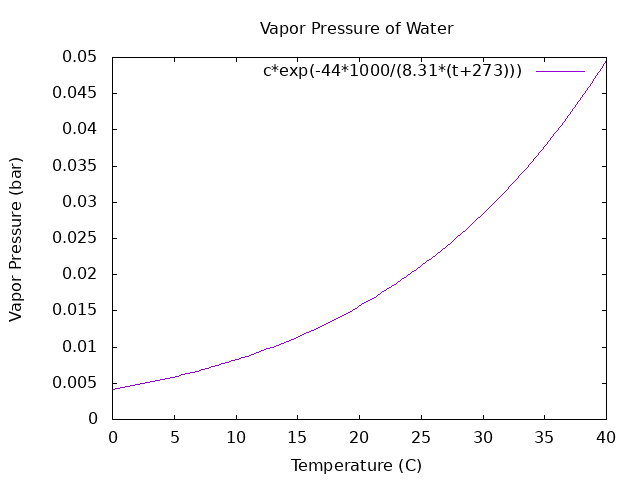
\includegraphics[scale=0.8]{dewpoint.png}\]
Indeed, vapor pressure appears to double every $\SI{10}{^{\circ}C}$

\section*{5.42b}
At $\SI{30}{^{\circ}C}$, the equillibrium vapor pressure appears to be about $\SI{0.025}{bar}$. At a relative humidity of $90\%$, this yields a partial pressure of water of $P=0.9(\SI{0.025}{bar})=\SI{0.0225}{bar}$. The dew point at this partial pressure appears fro the graph to be around $\SI{27}{^{\circ}C}$. If the relative humidity is $40\%$, the partial pressure is $\SI{0.01}{bar}$. This corresponds to a dewpoint, from inspection of the graph, of around $\SI{13}{^{\circ}C}$.

\section*{5.46a}
Since the chemical potential is the Gibbs free energy per molecule, the total Gibbs free energy is
\[G=N_{l}\mu_{l}+(N-N_{l})\mu_{v}\]
The total volume of the droplet is
\[V=\frac{4}{3}\pi r^{3}\]
We may therefore write the number of molecules in terms of the molecules per volume as
\[N_{l}=\frac{V}{v_{l}}=\frac{4\pi}{3}\frac{r^{3}}{v_{l}}\]

\section*{5.46b}
The surface area of the droplet is $A=4\pi r^{2}$. By the formula for surface tension, the new Gibbs free energy is
\[G=N_{l}\mu_{l}+(N-N_{l})\mu_{v}+4\pi\sigma r^{2}\]
\[=\frac{4\pi}{3}\frac{r^{3}}{v_{l}}\mu_{l}+\left( N-\frac{4\pi}{3}\frac{r^{3}}{v_{l}} \right)\mu_{v}+4\pi\sigma r^{2}\]

\section*{5.46c}
When the liquid chemical potential is large, we can drop the vapor term to get a rough estimate of the behavior of the Gibbs free energy with radius. This is plotted below.
\[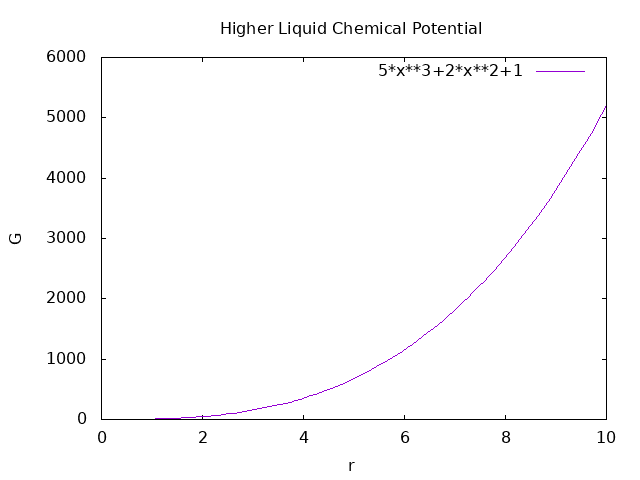
\includegraphics[scale=.8]{nucleation1.png}\]
In this case, there will be a stable equillibrium at zero, and the size of the droplet will decrease until it's fully evaporated.
When the liquid chemical potential is small, we may drop it instead, obtaining
\[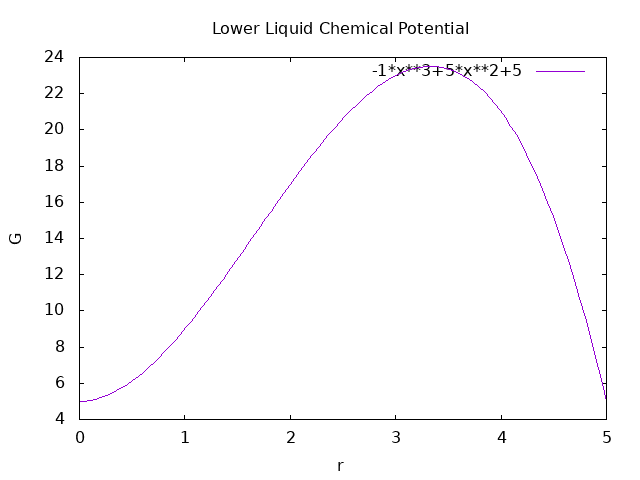
\includegraphics[scale=.8]{nucleation2.png}\]
Now, there is an equillibrium at some positive value, albeit an unstable one. In this case, the droplets will evaporate away if they are to the left of the maximum and experience runaway growth (until the assumptions fail) if they are to the right of it.

\section*{5.46d}
Since the Gibbs free energy tends to be minimized, we are looking for the $r$ that minimizes $G$.
\[G=\frac{4\pi}{3}\frac{r^{3}}{v_{l}}\mu_{l}+\left( N-\frac{4\pi}{3}\frac{r^{3}}{v_{l}} \right)\mu_{v}+4\pi\sigma r^{2}\]
has derivative
\[G'=4\pi r^{2}\mu_{l}/v_l-4\pi r^{2}\mu_{v}/v_{l}+8\pi\sigma r=\frac{4\pi r^{2}}{v_{l}}\left( \mu_{l}-\mu_{v} \right)+8\pi\sigma r\]
and therefore critical points at
\[\frac{4\pi r^{2}}{v_{l}}(\mu_{v}-\mu_{l})=8\pi\sigma r\Leftrightarrow r=\frac{2\sigma v_{l}}{\mu_{v}-\mu_{l}}\]
By the formula for the chemical potential of an ideal gas in terms of partial pressure,
\[\mu_{v}=\mu_{v}^{\circ}+kT\ln\left( \frac{P}{P^{\circ}} \right)\]
The relative humidity is the fraction by which the partial pressure of a gas is above its equillibrium pressure, so if we take $P^{\circ}$ to be that equillibrium pressure, the argument of the logarithm is merely the relative humidity $r$ and the reference chemical potential is the chemical potential of the liquid.
Therefore, we may write the critical radius as
\[r_{c}=\frac{2\sigma v_{l}}{kT\ln r}\]
At $\SI{20}{^{\circ}C}$ and atmospheric pressure, the coefficient of the inverse logarithm is
\[\frac{2\sigma v_{l}}{kT}=\frac{2(\SI{0.073}{J/m^{2}})[(\SI{1e-6}{m^{3}/cm^{3}})(\SI{1}{cm^{3}/g})(\SI{18}{g/mol})/(\SI{6.02e23}{particles/mol})]}{(\SI{1.38e-23}{J/K})(\SI{293}{K})}\]
\[=\SI{1.08e-9}{m}\]
A numerically accurate graph of this function appears below.
\[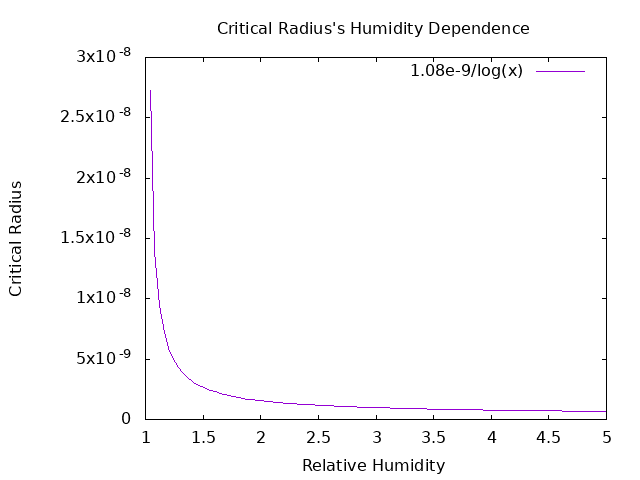
\includegraphics[scale=.8]{nucleation3.png}\]
The atmosphere is very rarely above $100\%$ humidity, so the critical radius value will remain in the neighborhood of 1 on the x-axis. Estimating the typical value at around $\SI{2e-8}{m}=\SI{20}{nm}$, by the argument above droplets smaller than this should evaporate. However, a $\SI{20}{nm}$ droplet is far too much water to ever form by random fluctuations alone, so it's unlikely clouds form spontaneously.

\section*{5.48}
The van der Waals equation for pressure as a function of volume is
\[P=\frac{NkT}{V-Nb}-\frac{aN^{2}}{V^{2}}\]
\[\Rightarrow \left( \frac{\partial P}{\partial V}\right)_{N,T}=\frac{2aN^{2}}{V^{3}}-\frac{NkT}{(V-Nb)^{2}}\]
\[\Rightarrow \left( \frac{\partial ^{2}P}{\partial V^{2}} \right)_{N,T}=\frac{2NkT}{(V-Nb)^{3}}-\frac{6aN^{2}}{V^{4}}\]
Setting these equal to zero, we obtain the sytsem
\[\frac{NkT}{(V-Nb)^{2}}=\frac{2aN^{2}}{V^{3}}\]
\[\frac{2NkT}{(V-Nb)^{3}}=\frac{6aN^{2}}{V^{4}}\]
Dividing the first by the second,
\[\frac{1}{2}(V-Nb)=\frac{1}{3}V\Rightarrow V_{c}=3Nb\]
this in to the original equation,
\[P_{c}=\frac{NkT}{3Nb-Nb}-\frac{aN^{2}}{9N^{2}b^{2}}=\frac{kT}{2b}-\frac{a}{9b^{2}}=\frac{9kbT-2a}{18b^{2}}\]
This would simplify further if we had the result for the critical temperature, so we plug the volume in to the first derivative critical point equation to obtain
\[\frac{NkT_{c}}{(3Nb-Nb)^{2}}=\frac{2aN^{2}}{27N^{3}b^{3}}\Leftrightarrow \frac{kT_{c}}{4Nb^{2}}=\frac{2a}{27Nb^{3}}
  \Leftrightarrow kT_{c}=\frac{8a}{27b}\]
Plugging this in to the incomplete critical pressure equation above,
\[P_{c}=\frac{9b(8a/27b)-2a}{18b^{2}}=\frac{8a/3-2a}{18b^{2}}=\frac{a}{27b^{2}}\]

\section*{5.55a}
The first two derivatives of the van der Waals equation with respect to volume were computed in the previous problem to be
\[P=\frac{NkT}{V-Nb}-\frac{aN^{2}}{V^{2}}\]
\[\Rightarrow \left( \frac{\partial P}{\partial V}\right)_{N,T}=\frac{2aN^{2}}{V^{3}}-\frac{NkT}{(V-Nb)^{2}}\]
\[\Rightarrow \left( \frac{\partial ^{2}P}{\partial V^{2}} \right)_{N,T}=\frac{2NkT}{(V-Nb)^{3}}-\frac{6aN^{2}}{V^{4}}\]
The third is clearly
\[\left( \frac{\partial^{3}P}{\partial V^{3}} \right)_{N,T}=\frac{24aN^{2}}{V^{5}}-\frac{6NkT}{(V-Nb)^{4}}\]
Evaluating these at $V_{c}$ and dividing by the factorial of the degree of derivative, the first four Taylor coefficients are
\[a_{0}=\frac{NkT}{V_{c}-Nb}-\frac{aN^{2}}{V_{c}^{2}}\]
\[a_{1}=\frac{2aN^{2}}{V_{c}^{2}}-\frac{NkT}{(V_{c}-Nb)^{2}}\]
\[a_{2}=\frac{NkT}{(V_{c}-Nb)^{3}}-\frac{3aN^{2}}{V_{c}^{4}}\]
\[a_{3}=\frac{4aN^{2}}{V^{5}_{c}}-\frac{NkT}{(V_{c}-Nb)^{4}}\]
The Taylor series is of course
\[P=a_{0}+a_{1}(V-V_{c})+a_{2}(V-V_{c})^{2}+a_{3}(V-V_{c})^{3}\]
Near $T_{c}$, $V_{c}\a$ %% TODO: argue this out

\section*{5.55b}
The curve being antisymmetric around $V=V_{c}$ implies the line that corrects the unphysical negative slopes of the $PV$ curve runs through $V_{c}$, since the antisymmetry implies that extending a horizontal line outwards will enclose equal areas. The pressure corresponding to $V_{c}$ is by our Taylor expansion
\[P=a_{0}=\frac{NkT}{V_{c}-Nb}-\frac{aN^{2}}{V_{c}^{2}}\]
This is a valid approximation in the neighborhood of the critical point, since the $PV$ diagram will be a horizontal line in that neighborhood.
This result is an expression for pressure in terms of temperature, as desired.
Differentiating it with respect to temperature yields a phase boundary slope of
\[\frac{dP}{dT}=\frac{Nk}{V_{c}-Nb}\]

\section*{5.56}
\[\frac{\partial S_{mixing}}{\partial x}=\frac{d}{dx}\left( -R\left[ x\ln x+(1-x)\ln(1-x) \right] \right)=-R\left( 1+\ln x+1+\ln(1-x) \right)\]
\[=-R(2+\ln(x-x^{2}))\]
The polynomial inside the logarithm has zeroes at $x=0$ and $x=1$, so the slope of the mixing entropy is infinite at those points.

\section{}
Under quasistatic expansion, the equation
\[W=-\int_{a}^{b}P(V)dV\]
holds. Therefore, we may calculate this work as
\[W=-\int_{V}^{2V}\left( \frac{NkT}{V-Nb}-\frac{aN^{2}}{V^{2}} \right)dV=-NkT\left( \ln(V-Nb)\bigg|_{V}^{2V} \right)+aN^{2}\left(-\frac{1}{V}\bigg|_{V}^{2V}  \right)\]
\[=-NkT\ln\left( \frac{2V-Nb}{V-Nb} \right)-aN^{2}\left(\frac{1}{2V}-\frac{1}{V} \right)=\frac{aN^{2}}{2V}-NkT\ln2\]

\section{}
The thermodynamic relation for enthalpy is
\[dH=TdS+VdP+\mu dN=TdS+ VdP\textrm{ (constant particles)}\]
Dividing through by $dP$,
\[\left( \frac{\partial H}{\partial P} \right)_{N,T}=T\left( \frac{\partial S}{\partial P} \right)_{N,T}+V\]
There is a Maxwell relation that $\left( \frac{\partial S}{\partial P} \right)_{N,T}=-\left( \frac{\partial V}{\partial T} \right)_{N,P}$, so we finally obtain
\[\left( \frac{\partial H}{\partial P} \right)_{N,T}=V-T\left( \frac{\partial V}{\partial T} \right)_{N,P}\]
For an ideal gas, this evaluates to
\[\left( \frac{\partial H}{\partial P} \right)_{N,T}=V-T\frac{\partial}{\partial T}\left( \frac{NkT}{P} \right)=V-\frac{NkT}{P}=0\]


The fundamental thermodynamic relation gives
\[dU=TdS-PdV+\mu dN=TdS-PdV\]
Dividing through by $dV$,
\[\left( \frac{\partial U}{\partial V}\right)_{N,T}=T\left( \frac{\partial S}{\partial V} \right)_{N,T}-P\]
There is a Maxwell relation that $\left( \frac{\partial S}{\partial V} \right)_{N,T}=\left( \frac{\partial P}{\partial T} \right)_{N,V}$, so we obtain
\[\left( \frac{\partial U}{\partial V} \right)_{N,T}=T\left( \frac{\partial P}{\partial T} \right)_{N,V}-P\]
For an ideal gas, this evaluates to
\[\left( \frac{\partial U}{\partial V} \right)_{N,T}=T\frac{\partial }{\partial T}\left(\frac{NkT}{V}  \right)-P=\frac{NkT}{V}-P=0\]


From a previous problem, we have
\[C_{P}=T\left( \frac{\partial S }{\partial T} \right)_{P}\]
Interchanging the differentiation, we may write,
\[\left( \frac{\partial C_{P}}{\partial P} \right)_{T}=T\left( \frac{\partial}{\partial T}\left( \frac{\partial S}{\partial P} \right)_{T} \right)_{P}\]
By a Maxwell relation,
\[=T\left( \frac{\partial}{\partial T}\left(-\frac{\partial V}{\partial T}  \right)_{P} \right)_{P}=-T\left( \frac{\partial ^{2}V}{\partial T^{2}} \right)_{P}\]
For an ideal gas,
\[\left( \frac{\partial C_{P}}{\partial P} \right)_{T}=-T\frac{\partial}{\partial T}\left( \frac{\partial }{\partial T}\left( \frac{NkT}{P} \right) \right)=0\]


\end{document}
%%% Local Variables:
%%% mode: latex
%%% TeX-master: t
%%% End:
